
\usetikzlibrary{backgrounds,circuits,circuits.ee.IEC,shapes,fit,matrix,automata,decorations.markings}
\UseTwocells

  \pgfdeclarelayer{edgelayer}
  \pgfdeclarelayer{nodelayer}
  \pgfsetlayers{edgelayer,nodelayer,main}

  \tikzset{font=\footnotesize}
  \tikzstyle{none}=[inner sep=0pt]

\tikzstyle{circ}=[circle,fill=black,draw,inner sep=3pt]
\tikzstyle{circ2}=[circle,fill=black,draw,inner sep=1pt]
  

  \tikzstyle{connection}=[circuit symbol open,
    circuit symbol size=width .5 height .5,
    shape=circle ee,
  inner sep=0.25\pgflinewidth]
  \tikzset{->-/.style={decoration={
    markings,
    mark=at position .54 with {\arrow{latex}}},postaction={decorate}}}

%%fakesubsubsection generators
\newcommand{\mult}[1]
{
\begin{aligned}
    \resizebox{#1}{!}{
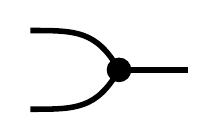
\begin{tikzpicture}
	\begin{pgfonlayer}{nodelayer}
		\node [style=none] (0) at (1, -0) {};
		\node [style=circ] (1) at (0.125, -0) {};
		\node [style=none] (2) at (-1, 0.5) {};
		\node [style=none] (3) at (-1, -0.5) {};
	\end{pgfonlayer}
	\begin{pgfonlayer}{edgelayer}
		\draw[line width=2pt] (0.center) to (1.center);
		\draw[line width=2pt] [in=0, out=120, looseness=1.20] (1.center) to (2.center);
		\draw[line width=2pt] [in=0, out=-120, looseness=1.20] (1.center) to (3.center);
	\end{pgfonlayer}
      \end{tikzpicture}}
\end{aligned}
}

\newcommand{\unit}[1]
{
  \begin{aligned}
    \resizebox{#1}{!}{

\begin{tikzpicture}
	\begin{pgfonlayer}{nodelayer}
		\node [style=none] (0) at (1, -0) {};
		\node [style=none] (1) at (-1, -0) {};
		\node [style=circ] (2) at (0, -0) {};
	\end{pgfonlayer}
	\begin{pgfonlayer}{edgelayer}
		\draw[line width=2pt] (0.center) to (2);
	\end{pgfonlayer}
      \end{tikzpicture}}
  \end{aligned}
}

\newcommand{\comult}[1]
{
\begin{aligned}
    \resizebox{#1}{!}{
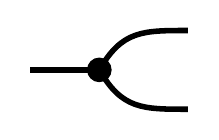
\begin{tikzpicture}
	\begin{pgfonlayer}{nodelayer}
		\node [style=none] (0) at (-1, -0) {};
		\node [style=circ] (1) at (-0.125, -0) {};
		\node [style=none] (2) at (1, 0.5) {};
		\node [style=none] (3) at (1, -0.5) {};
	\end{pgfonlayer}
	\begin{pgfonlayer}{edgelayer}
		\draw[line width=2pt] (0.center) to (1.center);
		\draw[line width=2pt] [in=180, out=60, looseness=1.20] (1.center) to (2.center);
		\draw[line width=2pt] [in=180, out=-60, looseness=1.20] (1.center) to (3.center);
	\end{pgfonlayer}
      \end{tikzpicture}}
\end{aligned}
}

\newcommand{\counit}[1]
{
  \begin{aligned}
    \resizebox{#1}{!}{

\begin{tikzpicture}
	\begin{pgfonlayer}{nodelayer}
		\node [style=none] (0) at (-1, -0) {};
		\node [style=none] (1) at (1, -0) {};
		\node [style=circ] (2) at (0, -0) {};
	\end{pgfonlayer}
	\begin{pgfonlayer}{edgelayer}
		\draw[line width=2pt] (0.center) to (2);
	\end{pgfonlayer}
      \end{tikzpicture}}
  \end{aligned}
}


\newcommand{\idone}[1]
{
  \begin{aligned}
    \resizebox{#1}{!}{
     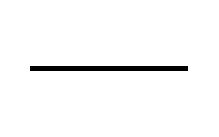
\begin{tikzpicture}
	\begin{pgfonlayer}{nodelayer}
		\node [style=none] (0) at (-1, -0) {};
		\node [style=none] (1) at (1, -0) {};
		\node [style=none] (2) at (0, 0.5) {};
		\node [style=none] (3) at (0, -0.5) {};
	\end{pgfonlayer}
	\begin{pgfonlayer}{edgelayer}
		\draw[line width=2pt] (1.center) to (0.center);
	\end{pgfonlayer}
\end{tikzpicture} 
    }
  \end{aligned}
}

\newcommand{\swap}[1]
{
  \begin{aligned}
    \resizebox{#1}{!}{
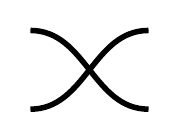
\begin{tikzpicture}
	\begin{pgfonlayer}{nodelayer}
		\node [style=none] (2) at (-0.5, -0.5) {};
		\node [style=none] (3) at (-2, 0.5) {};
		\node [style=none] (4) at (-0.5, 0.5) {};
		\node [style=none] (5) at (-2, -0.5) {};
	\end{pgfonlayer}
	\begin{pgfonlayer}{edgelayer}
		\draw[line width=2pt] [in=180, out=0, looseness=1.00] (3.center) to (2.center);
		\draw[line width=2pt] [in=0, out=180, looseness=1.00] (4.center) to (5.center);
	\end{pgfonlayer}
\end{tikzpicture}
    }
  \end{aligned}
}
%%fakesubsubsection associativity
\newcommand{\assocl}[1]
{
  \begin{aligned}
    \resizebox{#1}{!}{
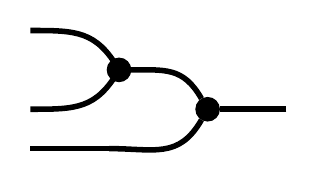
\begin{tikzpicture}
	\begin{pgfonlayer}{nodelayer}
		\node [style=circ] (0) at (0.125, -0) {};
		\node [style=none] (1) at (-1, 0.5) {};
		\node [style=none] (2) at (-1, -0.5) {};
		\node [style=none] (3) at (0, -1) {};
		\node [style=none] (4) at (2.25, -0.5) {};
		\node [style=none] (5) at (0.25, -0) {};
		\node [style=circ] (6) at (1.25, -0.5) {};
		\node [style=none] (7) at (-1, -1) {};
	\end{pgfonlayer}
	\begin{pgfonlayer}{edgelayer}
		\draw[line width=2pt] [in=0, out=120, looseness=1.20] (0.center) to (1.center);
		\draw[line width=2pt] [in=0, out=-120, looseness=1.20] (0.center) to (2.center);
		\draw[line width=2pt] (4.center) to (6);
		\draw[line width=2pt] [in=0, out=120, looseness=1.20] (6) to (5.center);
		\draw[line width=2pt] [in=0, out=-120, looseness=1.20] (6) to (3.center);
		\draw[line width=2pt] (3.center) to (7.center);
	\end{pgfonlayer}
      \end{tikzpicture}}
  \end{aligned}
}


\newcommand{\assocr}[1]
{
  \begin{aligned}
    \resizebox{#1}{!}{
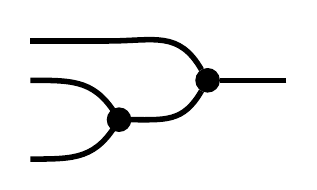
\begin{tikzpicture}
	\begin{pgfonlayer}{nodelayer}
		\node [style=circ] (0) at (0.125, -0.5) {};
		\node [style=none] (1) at (-1, -1) {};
		\node [style=none] (2) at (-1, 0) {};
		\node [style=none] (3) at (0, 0.5) {};
		\node [style=none] (4) at (2.25, 0) {};
		\node [style=none] (5) at (0.25, -0.5) {};
		\node [style=circ] (6) at (1.25, 0) {};
		\node [style=none] (7) at (-1, 0.5) {};
	\end{pgfonlayer}
	\begin{pgfonlayer}{edgelayer}
		\draw[line width=2pt] [in=0, out=-120, looseness=1.20] (0.center) to (1.center);
		\draw[line width=2pt] [in=0, out=120, looseness=1.20] (0.center) to (2.center);
		\draw[line width=2pt] (4.center) to (6);
		\draw[line width=2pt] [in=0, out=-120, looseness=1.20] (6) to (5.center);
		\draw[line width=2pt] [in=0, out=120, looseness=1.20] (6) to (3.center);
		\draw[line width=2pt] (3.center) to (7.center);
	\end{pgfonlayer}
      \end{tikzpicture}}
  \end{aligned}
}


\newcommand{\coassocl}[1]
{
  \begin{aligned}
    \resizebox{#1}{!}{
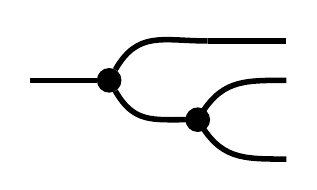
\begin{tikzpicture}
	\begin{pgfonlayer}{nodelayer}
		\node [style=circ] (0) at (1.125, -0.5) {};
		\node [style=none] (1) at (2.25, -1) {};
		\node [style=none] (2) at (2.25, 0) {};
		\node [style=none] (3) at (1.25, 0.5) {};
		\node [style=none] (4) at (-1, 0) {};
		\node [style=none] (5) at (1, -0.5) {};
		\node [style=circ] (6) at (0, 0) {};
		\node [style=none] (7) at (2.25, 0.5) {};
	\end{pgfonlayer}
	\begin{pgfonlayer}{edgelayer}
		\draw[line width=2pt] [in=180, out=-60, looseness=1.20] (0.center) to (1.center);
		\draw[line width=2pt] [in=180, out=60, looseness=1.20] (0.center) to (2.center);
		\draw[line width=2pt] (4.center) to (6);
		\draw[line width=2pt] [in=180, out=-60, looseness=1.20] (6) to (5.center);
		\draw[line width=2pt] [in=180, out=60, looseness=1.20] (6) to (3.center);
		\draw[line width=2pt] (3.center) to (7.center);
	\end{pgfonlayer}
      \end{tikzpicture}}
  \end{aligned}
}


\newcommand{\coassocr}[1]
{
  \begin{aligned}
    \resizebox{#1}{!}{
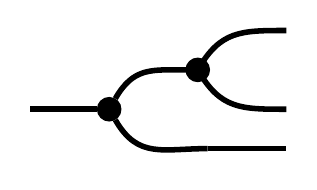
\begin{tikzpicture}
	\begin{pgfonlayer}{nodelayer}
		\node [style=circ] (0) at (1.125, 0) {};
		\node [style=none] (1) at (2.25, 0.5) {};
		\node [style=none] (2) at (2.25, -0.5) {};
		\node [style=none] (3) at (1.25, -1) {};
		\node [style=none] (4) at (-1, -0.5) {};
		\node [style=none] (5) at (1, 0) {};
		\node [style=circ] (6) at (0, -0.5) {};
		\node [style=none] (7) at (2.25, -1) {};
	\end{pgfonlayer}
	\begin{pgfonlayer}{edgelayer}
		\draw[line width=2pt] [in=180, out=60, looseness=1.20] (0.center) to (1.center);
		\draw[line width=2pt] [in=180, out=-60, looseness=1.20] (0.center) to (2.center);
		\draw[line width=2pt] (4.center) to (6);
		\draw[line width=2pt] [in=180, out=60, looseness=1.20] (6) to (5.center);
		\draw[line width=2pt] [in=180, out=-60, looseness=1.20] (6) to (3.center);
		\draw[line width=2pt] (3.center) to (7.center);
	\end{pgfonlayer}
      \end{tikzpicture}}
  \end{aligned}
}

%%fakesubsubsection unitality
\newcommand{\unitl}[1]
{
  \begin{aligned}
    \resizebox{#1}{!}{
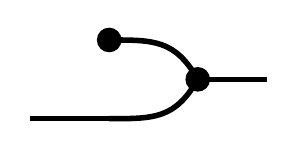
\begin{tikzpicture}
	\begin{pgfonlayer}{nodelayer}
		\node [style=none] (0) at (1, -0) {};
		\node [style=circ] (1) at (0.125, -0) {};
		\node [style=circ] (2) at (-1, 0.5) {};
		\node [style=none] (3) at (-1, -0.5) {};
		\node [style=none] (4) at (-2, -0.5) {};
	\end{pgfonlayer}
	\begin{pgfonlayer}{edgelayer}
		\draw[line width=2pt] (0.center) to (1.center);
		\draw[line width=2pt] [in=0, out=120, looseness=1.20] (1.center) to (2.center);
		\draw[line width=2pt] [in=0, out=-120, looseness=1.20] (1.center) to (3.center);
		\draw[line width=2pt] (4.center) to (3.center);
	\end{pgfonlayer}
\end{tikzpicture}
    }
  \end{aligned}
}

\newcommand{\counitl}[1]
{
  \begin{aligned}
    \resizebox{#1}{!}{
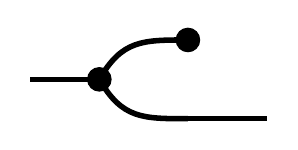
\begin{tikzpicture}
	\begin{pgfonlayer}{nodelayer}
		\node [style=none] (0) at (-2, -0) {};
		\node [style=circ] (1) at (-1.125, -0) {};
		\node [style=circ] (2) at (0, 0.5) {};
		\node [style=none] (3) at (0, -0.5) {};
		\node [style=none] (4) at (1, -0.5) {};
	\end{pgfonlayer}
	\begin{pgfonlayer}{edgelayer}
		\draw[line width=2pt] (0.center) to (1.center);
		\draw[line width=2pt] [in=180, out=60, looseness=1.20] (1.center) to (2.center);
		\draw[line width=2pt] [in=180, out=-60, looseness=1.20] (1.center) to (3.center);
		\draw[line width=2pt] (4.center) to (3.center);
	\end{pgfonlayer}
\end{tikzpicture}
    }
  \end{aligned}
}

%%fakesubsubsection commutativity
\newcommand{\commute}[1]
{
  \begin{aligned}
    \resizebox{#1}{!}{
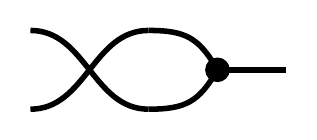
\begin{tikzpicture}
	\begin{pgfonlayer}{nodelayer}
		\node [style=none] (0) at (1.25, -0) {};
		\node [style=circ] (1) at (0.375, -0) {};
		\node [style=none] (2) at (-0.5, -0.5) {};
		\node [style=none] (3) at (-2, 0.5) {};
		\node [style=none] (4) at (-0.5, 0.5) {};
		\node [style=none] (5) at (-2, -0.5) {};
	\end{pgfonlayer}
	\begin{pgfonlayer}{edgelayer}
		\draw[line width=2pt] (0.center) to (1.center);
		\draw[line width=2pt] [in=0, out=-120, looseness=1.20] (1.center) to (2.center);
		\draw[line width=2pt] [in=180, out=0, looseness=1.00] (3.center) to (2.center);
		\draw[line width=2pt] [in=0, out=120, looseness=1.20] (1.center) to (4.center);
		\draw[line width=2pt] [in=0, out=180, looseness=1.00] (4.center) to (5.center);
	\end{pgfonlayer}
\end{tikzpicture}
    }
  \end{aligned}
}


\newcommand{\cocommute}[1]
{
  \begin{aligned}
    \resizebox{#1}{!}{
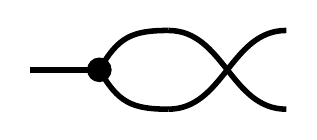
\begin{tikzpicture}
	\begin{pgfonlayer}{nodelayer}
		\node [style=none] (0) at (-2, -0) {};
		\node [style=circ] (1) at (-1.125, -0) {};
		\node [style=none] (2) at (-0.25, -0.5) {};
		\node [style=none] (3) at (1.25, 0.5) {};
		\node [style=none] (4) at (-0.25, 0.5) {};
		\node [style=none] (5) at (1.25, -0.5) {};
	\end{pgfonlayer}
	\begin{pgfonlayer}{edgelayer}
		\draw[line width=2pt] (0.center) to (1.center);
		\draw[line width=2pt] [in=180, out=-60, looseness=1.20] (1.center) to (2.center);
		\draw[line width=2pt] [in=0, out=180, looseness=1.00] (3.center) to (2.center);
		\draw[line width=2pt] [in=180, out=60, looseness=1.20] (1.center) to (4.center);
		\draw[line width=2pt] [in=180, out=0, looseness=1.00] (4.center) to (5.center);
	\end{pgfonlayer}
\end{tikzpicture}
    }
  \end{aligned}
}
%%fakesubsubsection frobenius


\newcommand{\frobs}[1]
{
  \begin{aligned}
    \resizebox{#1}{!}{
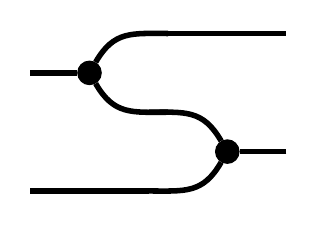
\begin{tikzpicture}
	\begin{pgfonlayer}{nodelayer}
		\node [style=none] (0) at (-1.5, 0.5) {};
		\node [style=circ] (1) at (-0.75, 0.5) {};
		\node [style=none] (2) at (0.25, -0) {};
		\node [style=none] (3) at (0.25, 1) {};
		\node [style=circ] (4) at (1, -0.5) {};
		\node [style=none] (5) at (0, -0) {};
		\node [style=none] (6) at (1.75, -0.5) {};
		\node [style=none] (7) at (0, -1) {};
		\node [style=none] (8) at (1.75, 1) {};
		\node [style=none] (9) at (-1.5, -1) {};
	\end{pgfonlayer}
	\begin{pgfonlayer}{edgelayer}
		\draw[line width=2pt] [in=180, out=-60, looseness=1.20] (1) to (2.center);
		\draw[line width=2pt] [in=180, out=60, looseness=1.20] (1) to (3.center);
		\draw[line width=2pt] (0.center) to (1);
		\draw[line width=2pt] (6.center) to (4);
		\draw[line width=2pt] [in=0, out=120, looseness=1.20] (4) to (5.center);
		\draw[line width=2pt] [in=0, out=-120, looseness=1.20] (4) to (7.center);
		\draw[line width=2pt] (3.center) to (8.center);
		\draw[line width=2pt] (7.center) to (9.center);
	\end{pgfonlayer}
\end{tikzpicture}
    }
  \end{aligned}
}

\newcommand{\frobx}[1]
{
  \begin{aligned}
    \resizebox{#1}{!}{
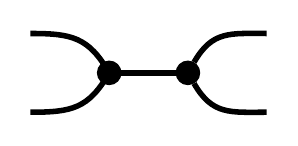
\begin{tikzpicture}
	\begin{pgfonlayer}{nodelayer}
		\node [style=circ] (0) at (-0.5, -0) {};
		\node [style=none] (1) at (-1.5, -0.5) {};
		\node [style=none] (2) at (-1.5, 0.5) {};
		\node [style=circ] (3) at (0.5, -0) {};
		\node [style=none] (4) at (1.5, -0.5) {};
		\node [style=none] (5) at (1.5, 0.5) {};
	\end{pgfonlayer}
	\begin{pgfonlayer}{edgelayer}
		\draw[line width=2pt] [in=0, out=-120, looseness=1.20] (0.center) to (1.center);
		\draw[line width=2pt] [in=0, out=120, looseness=1.20] (0.center) to (2.center);
		\draw[line width=2pt] [in=180, out=-60, looseness=1.20] (3) to (4.center);
		\draw[line width=2pt] [in=180, out=60, looseness=1.20] (3) to (5.center);
		\draw[line width=2pt] (0) to (3);
	\end{pgfonlayer}
\end{tikzpicture}
    }
  \end{aligned}
}

\newcommand{\frobz}[1]
{
  \begin{aligned}
    \resizebox{#1}{!}{
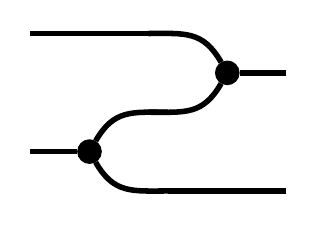
\begin{tikzpicture}
	\begin{pgfonlayer}{nodelayer}
		\node [style=none] (0) at (1.75, 0.5) {};
		\node [style=circ] (1) at (1, 0.5) {};
		\node [style=none] (2) at (0, -0) {};
		\node [style=none] (3) at (0, 1) {};
		\node [style=circ] (4) at (-0.75, -0.5) {};
		\node [style=none] (5) at (0.25, -0) {};
		\node [style=none] (6) at (-1.5, -0.5) {};
		\node [style=none] (7) at (0.25, -1) {};
		\node [style=none] (8) at (-1.5, 1) {};
		\node [style=none] (9) at (1.75, -1) {};
	\end{pgfonlayer}
	\begin{pgfonlayer}{edgelayer}
		\draw[line width=2pt] [in=0, out=-120, looseness=1.20] (1) to (2.center);
		\draw[line width=2pt] [in=0, out=120, looseness=1.20] (1) to (3.center);
		\draw[line width=2pt] (0.center) to (1);
		\draw[line width=2pt] (6.center) to (4);
		\draw[line width=2pt] [in=180, out=60, looseness=1.20] (4) to (5.center);
		\draw[line width=2pt] [in=180, out=-60, looseness=1.20] (4) to (7.center);
		\draw[line width=2pt] (3.center) to (8.center);
		\draw[line width=2pt] (7.center) to (9.center);
	\end{pgfonlayer}
\end{tikzpicture}
    }
  \end{aligned}
}
%%fakesubsubsection bimonoid

\newcommand{\bi}[1]
{
  \begin{aligned}
    \resizebox{#1}{!}{
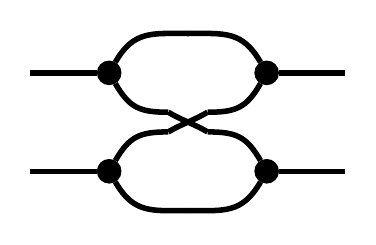
\begin{tikzpicture}
	\begin{pgfonlayer}{nodelayer}
		\node [style=none] (0) at (-2, 0.75) {};
		\node [style=none] (1) at (-2, -0.5) {};
		\node [style=circ] (2) at (-1, 0.75) {};
		\node [style=circ] (3) at (-1, -0.5) {};
		\node [style=none] (4) at (0, 1.25) {};
		\node [style=none] (5) at (-0.25, 0.25) {};
		\node [style=none] (6) at (-0.25, -0) {};
		\node [style=none] (7) at (0, -1) {};
		\node [style=none] (8) at (0, 1.25) {};
		\node [style=none] (9) at (0.25, 0.25) {};
		\node [style=none] (10) at (0.25, -0) {};
		\node [style=none] (11) at (0, -1) {};
		\node [style=circ] (12) at (1, 0.75) {};
		\node [style=circ] (13) at (1, -0.5) {};
		\node [style=none] (14) at (2, 0.75) {};
		\node [style=none] (15) at (2, -0.5) {};
	\end{pgfonlayer}
	\begin{pgfonlayer}{edgelayer}
		\draw[line width=2pt] (0.center) to (2);
		\draw[line width=2pt] (1.center) to (3);
		\draw[line width=2pt] (12) to (14.center);
		\draw[line width=2pt] (13) to (15.center);
		\draw[line width=2pt] [in=180, out=60, looseness=1.20] (2) to (4.center);
		\draw[line width=2pt] [in=180, out=-60, looseness=1.20] (2) to (5.center);
		\draw[line width=2pt] [in=180, out=60, looseness=1.20] (3) to (6.center);
		\draw[line width=2pt] [in=180, out=-60, looseness=1.20] (3) to (7.center);
		\draw[line width=2pt] [in=120, out=0, looseness=1.20] (8.center) to (12);
		\draw[line width=2pt] [in=-120, out=0, looseness=1.20] (9.center) to (12);
		\draw[line width=2pt] [in=120, out=0, looseness=1.20] (10.center) to (13);
		\draw[line width=2pt] [in=-120, out=0, looseness=1.20] (11.center) to (13);
		\draw[line width=2pt] (4.center) to (8.center);
		\draw[line width=2pt] [in=150, out=-30, looseness=1.00] (5.center) to (10.center);
		\draw[line width=2pt] [in=-150, out=30, looseness=1.00] (6.center) to (9.center);
		\draw[line width=2pt] (7.center) to (11.center);
	\end{pgfonlayer}
\end{tikzpicture}
    }
  \end{aligned}
}

\newcommand{\bimultl}[1]
{
\begin{aligned}
    \resizebox{#1}{!}{
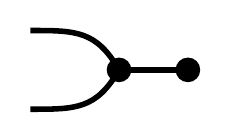
\begin{tikzpicture}
	\begin{pgfonlayer}{nodelayer}
		\node [style=circ] (0) at (1, -0) {};
		\node [style=circ] (1) at (0.125, -0) {};
		\node [style=none] (2) at (-1, 0.5) {};
		\node [style=none] (3) at (-1, -0.5) {};
	\end{pgfonlayer}
	\begin{pgfonlayer}{edgelayer}
		\draw[line width=2pt] (0.center) to (1.center);
		\draw[line width=2pt] [in=0, out=120, looseness=1.20] (1.center) to (2.center);
		\draw[line width=2pt] [in=0, out=-120, looseness=1.20] (1.center) to (3.center);
	\end{pgfonlayer}
      \end{tikzpicture}}
\end{aligned}
}

\newcommand{\bimultr}[1]
{
\begin{aligned}
    \resizebox{#1}{!}{
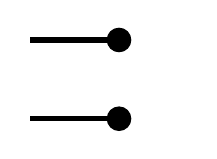
\begin{tikzpicture}
	\begin{pgfonlayer}{nodelayer}
		\node [style=none] (e) at (1, -0) {};
		\node [style=circ] (0) at (0.125, 0.5) {};
		\node [style=circ] (1) at (0.125, -0.5) {};
		\node [style=none] (2) at (-1, 0.5) {};
		\node [style=none] (3) at (-1, -0.5) {};
	\end{pgfonlayer}
	\begin{pgfonlayer}{edgelayer}
		\draw[line width=2pt] (2.center) to (0.center);
		\draw[line width=2pt] (3.center) to (1.center);
	\end{pgfonlayer}
      \end{tikzpicture}}
\end{aligned}
}

\newcommand{\bicomultl}[1]
{
\begin{aligned}
    \resizebox{#1}{!}{
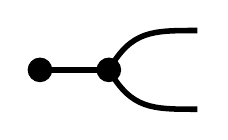
\begin{tikzpicture}
	\begin{pgfonlayer}{nodelayer}
		\node [style=circ] (0) at (-1, -0) {};
		\node [style=circ] (1) at (-0.125, -0) {};
		\node [style=none] (2) at (1, 0.5) {};
		\node [style=none] (3) at (1, -0.5) {};
	\end{pgfonlayer}
	\begin{pgfonlayer}{edgelayer}
		\draw[line width=2pt] (0.center) to (1.center);
		\draw[line width=2pt] [in=180, out=60, looseness=1.20] (1.center) to (2.center);
		\draw[line width=2pt] [in=180, out=-60, looseness=1.20] (1.center) to (3.center);
	\end{pgfonlayer}
      \end{tikzpicture}}
\end{aligned}
}

\newcommand{\bicomultr}[1]
{
\begin{aligned}
    \resizebox{#1}{!}{
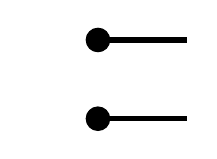
\begin{tikzpicture}
	\begin{pgfonlayer}{nodelayer}
		\node [style=none] (e) at (-1, -0) {};
		\node [style=circ] (0) at (-0.125, 0.5) {};
		\node [style=circ] (1) at (-0.125, -0.5) {};
		\node [style=none] (2) at (1, 0.5) {};
		\node [style=none] (3) at (1, -0.5) {};
	\end{pgfonlayer}
	\begin{pgfonlayer}{edgelayer}
		\draw[line width=2pt] (0.center) to (2.center);
		\draw[line width=2pt] (1.center) to (3.center);
	\end{pgfonlayer}
      \end{tikzpicture}}
\end{aligned}
}
%%fakesubsubsection speciality

\newcommand{\spec}[1]
{
  \begin{aligned}
    \resizebox{#1}{!}{
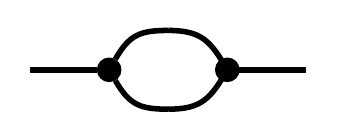
\begin{tikzpicture}
	\begin{pgfonlayer}{nodelayer}
		\node [style=none] (0) at (1.75, -0) {};
		\node [style=circ] (1) at (0.75, -0) {};
		\node [style=none] (2) at (0, -0.5) {};
		\node [style=none] (3) at (0, 0.5) {};
		\node [style=circ] (4) at (-0.75, -0) {};
		\node [style=none] (5) at (0, -0.5) {};
		\node [style=none] (6) at (-1.75, -0) {};
		\node [style=none] (7) at (0, 0.5) {};
	\end{pgfonlayer}
	\begin{pgfonlayer}{edgelayer}
		\draw[line width=2pt] (0.center) to (1.center);
		\draw[line width=2pt] [in=0, out=-120, looseness=1.20] (1.center) to (2.center);
		\draw[line width=2pt] [in=0, out=120, looseness=1.20] (1.center) to (3.center);
		\draw[line width=2pt] (6.center) to (4);
		\draw[line width=2pt] [in=180, out=-60, looseness=1.20] (4) to (5.center);
		\draw[line width=2pt] [in=180, out=60, looseness=1.20] (4) to (7.center);
	\end{pgfonlayer}
\end{tikzpicture}
    }
  \end{aligned}
}

\newcommand{\extral}[1]
{
  \begin{aligned}
    \resizebox{#1}{!}{

\begin{tikzpicture}
	\begin{pgfonlayer}{nodelayer}
		\node [style=none] (0) at (1.75, -0) {};
		\node [style=circ] (1) at (0.75, -0) {};
		\node [style=circ] (4) at (-0.75, -0) {};
		\node [style=none] (6) at (-1.75, -0) {};
	\end{pgfonlayer}
	\begin{pgfonlayer}{edgelayer}
	  \draw[line width=2pt] (1.center) to (4.center);
	\end{pgfonlayer}
\end{tikzpicture}
    }
  \end{aligned}
}

\newcommand{\extrar}[1]
{
  \begin{aligned}
    \resizebox{#1}{!}{
\begin{tikzpicture}
	\begin{pgfonlayer}{nodelayer}
		\node [style=none] (0) at (1.75, -0) {};
		\node [style=none] (6) at (-1.75, -0) {};
	\end{pgfonlayer}
\end{tikzpicture}
    }
  \end{aligned}
}




